

%--------------------------------------------------------------------
\section{Antecedentes}
La Secretaría del Medio Ambiente del Distrito Federal cuenta con un sistema informático que maneja la información referente a los residuos sólidos. 
\\\\
El SIRS se desarrolló con el propósito de manejar y analizar, de manera sistemática, la información disponible en materia de residuos sólidos para apoyar acciones en la planeación, desarrollo de infraestructura de tratamiento, disposición de residuos y de investigación en el área de residuos sólidos, así como de proporcionar información confiable y actualizada a la ciudadana a través del Inventario de Residuos Sólidos del Distrito Federal.





%--------------------------------------------------------------------
\section{Descripción de la problemática}
El Software SIRS no lleva a cabo diferentes procesos que son indispensables para la Secretaría del Medio Ambiente del Distrito Federal, entre estos procesos están:
\begin{itemize}
	\item Generar un reporte que contenga información como: Total recolectado, por colonia, delegación, vehículo, chofer. de forma diaria, mensual, semanal o anual.
	\item La ruta no está plenamente identificada con las colonias, unidades habitacionales, negocios, mercados, etc.
	\item El sistema no contempla que los vehículos de recolección transportan toda la basura a las estaciones de transferencia y, posteriormente, los residuos se trasladan en vehículos Transfer a sitios de disposición final.
\end{itemize}

También tiene los siguientes problemas

\begin{itemize}
	\item Los reportes que genera el sistema están limitados a un formato fijo y no se permite eliminar o agregar campos para datos relevantes  según la necesidad de cada reporte por lo cual no existe la  personalización de los reportes. 
	\item Existen problemas de consistencia en la información.
	\item El sistema no ofrece interacción con otros sistemas.
\end{itemize}
Lo anterior hace que la Secretaría considere que el sistema debe rehacerse o mejorarse sustancialmente.


%--------------------------------------------------------------------
\section{Soluciones en el mercado}
\begin{figure}[h!]
	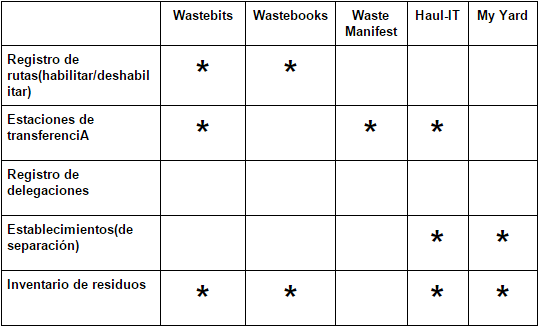
\includegraphics[width=13cm, height=6.5cm]{tabla.PNG}
\end{figure}

Para la problemática que se nos presenta se revisaron las diferentes opciones que existen en el mercado, esto con la finalidad  de poder tener como  posibilidad  el ahorro de un   gasto en el desarrollo de un sistema nuevo  y optar  en este caso por  la compra de la licencia de un software, pero al ver que estos softwares no cumplen con las necesidades a cubrir totalmente o en su mayoría, la opción más viable actualmente es el desarrollo de un sistema a la medida 

%--------------------------------------------------------------------
\section{Propuesta de solución}
Tras analizar la problemática se propone:
\begin{itemize}
	\item Rehacer el sistema actual partiendo de la estructura que actualmente ya maneja añadiendo los procesos con los que no cuenta descritos en la problemática. 
	\item Unificar todas las tecnologías de los otros sistemas para su posterior integración.
\end{itemize}



%--------------------------------------------------------------------
\section{Beneficios esperados}
\begin{itemize}
	\item Ayudar a la secretaría del Medio Ambiente del Distrito Federal a tener una mejor gestión de la información sobre las recolecciones que se realizan dependiendo las delegaciones en las cuales se realizan generando diferentes tipos de informes.
	
	\item Ayudar a la secretaría del Medio Ambiente del Distrito Federal a tener una una gestión de manera más clara de la información sobre las recolecciones que se realizan dependiendo las delegaciones mediante la obtención de ruta, chofer, vehiculo, cantidad de residuos recolectados por vuelta, y poder generar un informe con estos datos ya sea por dia, semana, mes o año.
	
	\item Reducir el tiempo y costo para la recopilación, transferencia y comunicación de información, debido a que se agilizarán los procesos de consulta y actualización.
	
	\item Facilitar el proceso de toma de decisiones como el correcto cobro de impuestos, instalacion de depositos de basura en lugares adecuados, asignar vehículos a las rutas que lo requieran, asignar correctamente el presupuesto a las delegaciones y premiar a los empleados que se lo merecen.
	
	\item Organizar la información para mejorar el proceso de acceso a la información pública, para la ciudadanía al momento de que se requieran consultar informes.
	
\end{itemize}
